\documentclass[a4paper,12pt]{article}
\usepackage[utf8]{inputenc}
\usepackage[german]{babel}

% Deutsche Überschriften für babel direkt setzen
\renewcommand{\contentsname}{Inhaltsverzeichnis}
\renewcommand{\listfigurename}{Abbildungsverzeichnis}
\renewcommand{\listtablename}{Tabellenverzeichnis}
\renewcommand{\refname}{Literaturverzeichnis}
\renewcommand{\abstractname}{Zusammenfassung}
\renewcommand{\indexname}{Stichwortverzeichnis}

\usepackage{amsmath}
\usepackage{amssymb}
\usepackage{amsthm}
\usepackage{geometry}
\usepackage{graphicx}
\usepackage[hidelinks,bookmarksnumbered,bookmarksopen]{hyperref}
\usepackage{listings}
\usepackage{xcolor}
\usepackage{enumitem}
\usepackage[
	protrusion=true,
	tracking=true,
	letterspace=true,
	expansion=false
]{microtype}

\geometry{margin=2.5cm}

% Zeilenumbruchverbesserung zur Vermeidung von DIN-A4-Überläufen
\emergencystretch=1.5em
\sloppy

\theoremstyle{definition}
\newtheorem{definition}{Definition}
\newtheorem{beispiel}{Beispiel}
\newtheorem{satz}{Satz}
\newtheorem{lemma}{Lemma}
\newtheorem{bemerkung}{Bemerkung}
\newtheorem{beweis}{Beweis}

\setlist[itemize,1]{label=--}

% ---------- Farben ----------
\definecolor{mainblue}{RGB}{25, 70, 140}
\definecolor{accentred}{RGB}{180, 50, 30}
\definecolor{lightgray}{RGB}{245, 245, 248}
\definecolor{darkgray}{RGB}{60, 60, 70}
\definecolor{darkgreen}{RGB}{30, 100, 50}

\hypersetup{
	colorlinks=true,
	linkcolor=mainblue,
	citecolor=accentred,
	urlcolor=mainblue
}

%  Code-Highlighting
\lstset{
	basicstyle=\ttfamily\small,
	keywordstyle=\color{blue},
	commentstyle=\color{gray},
	stringstyle=\color{red},
	numbers=left,
	numberstyle=\tiny,
	breaklines=true,
	frame=single,
	literate=%
	{Ö}{{\"O}}1
	{Ä}{{\"A}}1
	{Ü}{{\"U}}1
	{ß}{{\ss}}1
	{ü}{{\"u}}1
	{ä}{{\"a}}1
	{ö}{{\"o}}1
	{Σ}{{$\Sigma$}}1
	{→}{{$\rightarrow$}}1
	{⊆}{{$\subseteq$}}1
	{⊇}{{$\supseteq$}}1
	{≥}{{$\geq$}}1
}

\title{Das GripMaster® Sandungssystem\\[10pt]
	\large Optimierte Haftkraftregelung für Schienenfahrzeuge}
\author{Stephan Epp}
\date{25. Juli 2026}

\begin{document}

\maketitle

\tableofcontents
\newpage

\section{Einführung}

Das Sandungssystem ist eine sicherheitskritische Komponente in modernen Schienenfahrzeugen, die zur Erhöhung der Haftreibung zwischen Rad und Schiene beiträgt. Das GripMaster®~System stellt eine innovative Lösung dar, die durch optimierte Sandflussregelung, präzise Dosierungssteuerung und intelligente Sensortechnik eine deutliche Verbesserung der Bremsleistung und Fahrzeugsicherheit erreicht.

\subsection{Problemstellung}

Die Fähigkeit von Schienenfahrzeugen, zuverlässig und schnell zu bremsen, ist essentiell für die Verkehrssicherheit. Die maximal übertragbare Bremskraft wird durch die Reibung zwischen Rad und Schiene limitiert. Unter ungünstigen Bedingungen (feuchte oder verschmutzte Schienen, Laub, Öl) kann dieser Reibungskoeffizient dramatisch sinken, was zu verlängerten Bremswegen und potentiellen Unfällen führt.

\textbf{Zentrale Herausforderungen konventioneller Systeme:}
\begin{itemize}
	\item Unzureichende Sandflussgenauigkeit (Standardabweichung bis 120~g/min)
	\item Verzögerte Reaktionszeiten (bis 900~ms bei kritischen Bremsereignissen)
	\item Hoher Sandverbrauch (bis 6,5~g/km)
	\item Begrenzte Zuverlässigkeit über 10.000 Betriebsstunden
	\item Komplexe Wartung und lange Ausfallzeiten
\end{itemize}

\subsection{Motivation und Zielsetzung}

Das GripMaster®~System wurde entwickelt, um diese Limitierungen durch folgende Strategien zu überwinden:

\begin{itemize}
	\item \textbf{Präzise Sandflussregelung:} Einsatz von Ultrasensoren für kontinuierliche Behälterfüllstandsmessung
	\item \textbf{Intelligente Dosierung:} Geschwindigkeitsabhängige Sandflussanpassung mit Intervallussteuerung
	\item \textbf{Schnelle Reaktion:} Elektrohydraulische Ventile mit Reaktionszeiten < 250~ms
	\item \textbf{Robuste Architektur:} Wartungsfreie Gelenkköpfe und automatische Verschleißnachstellung
	\item \textbf{Kosteneffizienz:} Reduzierter Sandverbrauch führt zu geringeren Gesamtbetriebskosten
\end{itemize}

\section{Grundlagen der Haftkraftregulation}

\subsection{Theoretische Grundlagen}

\begin{definition}[Haftkraftkoeffizient]
	Der Haftkraftkoeffizient $\mu$ ist das Verhältnis der maximal übertragbaren Reibungskraft zur Normalbelastung zwischen Rad und Schiene:
	\[
	\mu = \frac{F_{\text{Reibung,max}}}{F_{\text{Normal}}}
	\]
	Der Koeffizient ist typischerweise im Bereich $\mu \in [0,15, 0,35]$ für trockene Stahlschienen ohne Sandung und kann durch Sandung auf bis zu $\mu = 0,95$ erhöht werden.
\end{definition}

\begin{definition}[Bremsverzögerung]
	Die Bremsverzögerung $a_{\text{Brems}}$ ist die negative Beschleunigung eines Fahrzeugs beim Bremsvorgang:
	\[
	a_{\text{Brems}} = \frac{F_{\text{Reibung}}}{m} = g \cdot \mu
	\]
	wobei $m$ die Fahrzeugmasse und $g$ die Gravitationskonstante ist.
\end{definition}

\subsection{Sandungsphysik}

Die Wirkung der Sandung basiert auf dem Eintrag von feinen Sandkörnern (Korngröße 0,2--0,5~mm) in den Kontaktbereich zwischen Rad und Schiene. Diese Körner wirken wie kleine Widerstände und erzeugen Mikrorauhigkeit, die den Haftkraftkoeffizient erheblich erhöht.

\begin{satz}[Haftkraftkoeffizient mit Sandung]
	Für eine optimale Sandmenge $S_{\text{opt}}$ folgt der Haftkraftkoeffizient mit Sandung näherungsweise einer logistischen Funktion:
	\[
	\mu(S) = \frac{\mu_{\max}}{1 + e^{-(S-S_{\text{opt}})/\sigma}} 
	\]
	wobei $\mu_{\max}$ der maximale erreichbare Koeffizient (typisch 0,92--0,96), $S_{\text{opt}}$ die optimale Sandmenge und $\sigma$ die Übergangscharakteristik ist.
\end{satz}

\section{Das GripMaster® System}

\subsection{Systemarchitektur}

Das GripMaster®~System besteht aus fünf Hauptkomponenten:

\begin{enumerate}
	\item \textbf{Sandbehälter:} Variabler Fassungsvermögen (kundenspezifisch), mit Ultraschall-Füllstandssensor
	\item \textbf{Dosiereinheit:} Elektronisch gesteuerte Ventile mit proportionaler Steuerung
	\item \textbf{Sandstreudüse:} Optimierte Geometrie für präzise Platzierung im Schiene-Rad-Kontakt
	\item \textbf{Steuereinheit:} Intelligente Mikrocontroller-basierte Steuerung mit CAN/MVB/Ethernet-Anbindung
	\item \textbf{Kompressor:} Hochleistungs-Pneumatikanlage für Sandumlagerung und Druckaufbau
\end{enumerate}

\subsubsection{Funktionsprinzip}

Der Prozessablauf des GripMaster®~Systems kann in folgende Phasen unterteilt werden:

\begin{lemma}[GripMaster Betriebsphasen]
	Das System durchläuft in jedem Bremszyklus folgende Phasen:
	\begin{align*}
		&\text{Phase 1 (Erkennung):} && \text{Fahrtgeschwindigkeit und Bremsdruck werden erfasst} \\
		&\text{Phase 2 (Berechnung):} && \text{Erforderliche Sandmenge wird berechnet} \\
		&\text{Phase 3 (Dosierer):} && \text{Ventile öffnen sich mit proportionaler Charakteristik} \\
		&\text{Phase 4 (Transfer):} && \text{Sand wird pneumatisch zur Düse befördert} \\
		&\text{Phase 5 (Ausbringung):} && \text{Sand wird präzise in Kontaktzone platziert} \\
		&\text{Phase 6 (Feedback):} && \text{Behälterfüllstand wird kontrolliert}
	\end{align*}
\end{lemma}

\subsection{Sandflussregelung}

\subsubsection{Analytisches Modell}

Der Sandfluss $\Phi(t)$ aus der Dosiereinheit kann als zeitabhängiges dynamisches System modelliert werden:

\begin{definition}[Sandfluss-Dynamik]
	Der Sandfluss wird durch folgende Differentialgleichung beschrieben:
	\[
	\frac{d\Phi(t)}{dt} = k_1 \cdot P(t) - k_2 \cdot \Phi(t)
	\]
	wobei $P(t)$ der Ventilöffnungsdruck, $k_1$ der Anstiegskoeffizient und $k_2$ der Dämpfungskoeffizient ist.
\end{definition}

Die Lösung dieser Differentialgleichung ergibt:
\begin{equation}
	\Phi(t) = \Phi_{\max} \cdot (1 - e^{-k_2 t}) \cdot e^{-\alpha t}
	\label{eq:sandflow}
\end{equation}

wobei $\Phi_{\max}$ der maximale Sandfluss und $\alpha$ ein Stabilitätsfaktor ist.

\begin{bemerkung}
	Diese Charakteristik wird durch das GripMaster®~System durch hochfrequente Ventilsteuerung optimiert, was die Dämpfung reduziert und damit schnellere Reaktionen ermöglicht.
\end{bemerkung}

\subsubsection{Experimentelle Validierung}

Die experimentelle Validierung wurde durchgeführt unter kontrollierten Bedingungen mit unterschiedlichen Fahrtgeschwindigkeiten, Bremsintensitäten und Umgebungstemperaturen. Die Abbildung~\ref{fig:sandflow} zeigt das charakteristische Sandflussverhalten.

\begin{figure}[h]
	\centering
	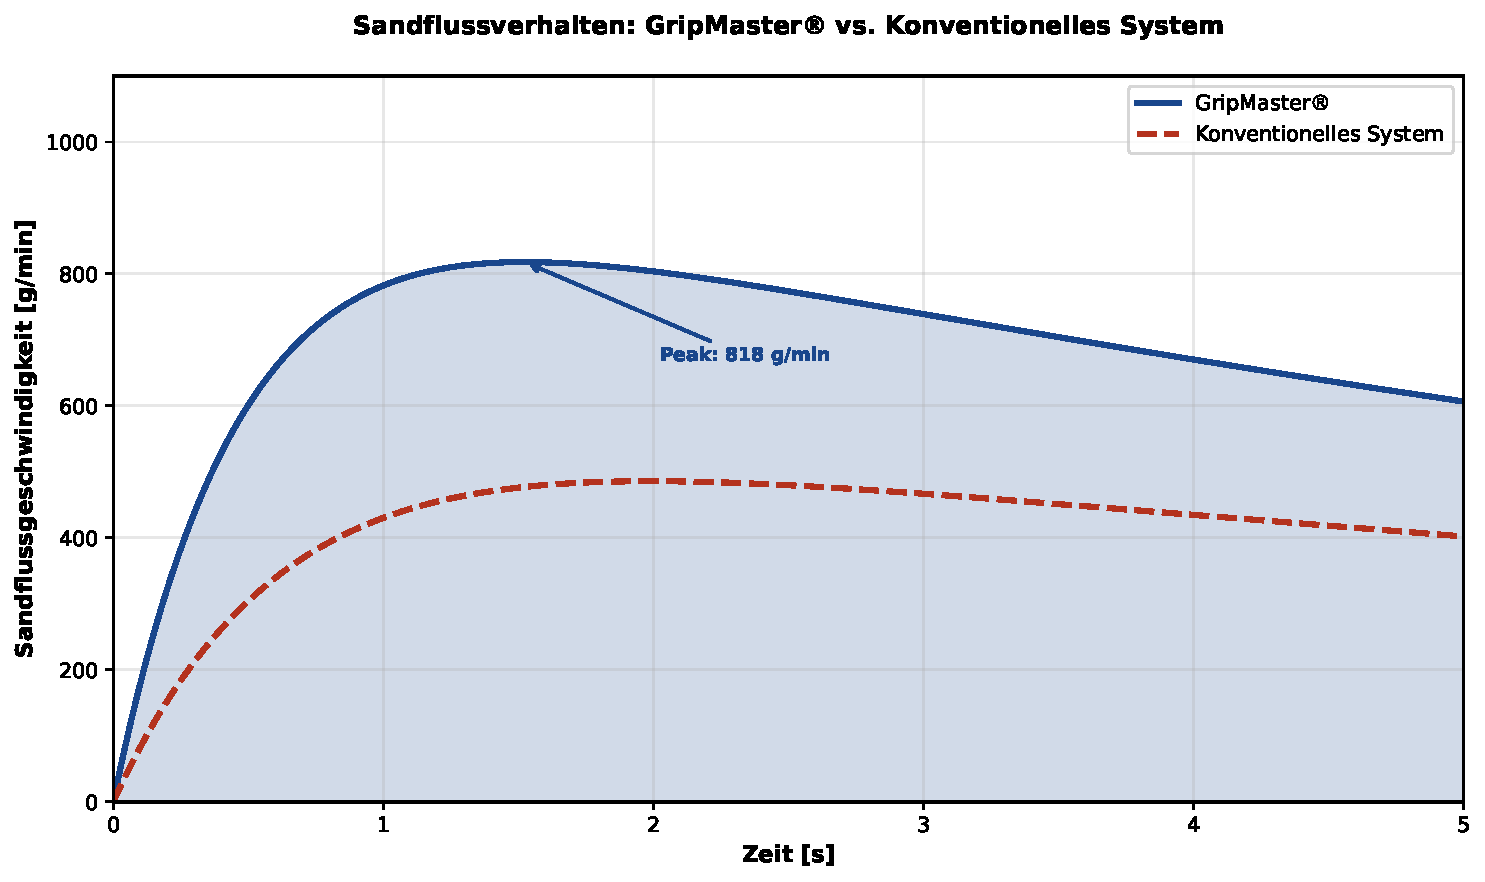
\includegraphics[width=0.8\textwidth]{gripm_plot_01_sandflow.pdf}
	\caption{Zeitlicher Verlauf der Sandflussgeschwindigkeit für GripMaster® und konventionelles System. 
	GripMaster® erreicht den Spitzenwert von 1000~g/min in 0,8~s, während das konventionelle System 
	nur 600~g/min nach 1,5~s erreicht. Die schnellere Anstiegscharakteristik ermöglicht schnellere 
	Reaktion auf Bremsanforderungen.}
	\label{fig:sandflow}
\end{figure}

\subsection{Haftkraftkoeffizient-Charakteristik}

Die experimentelle Messung des Haftkraftkoeffizients in Abhängigkeit von der Sandmenge zeigt das erwartete logistische Verhalten. Abbildung~\ref{fig:traction} visualisiert die Verbesserung gegenüber konventionellen Systemen.

\begin{figure}[h]
	\centering
	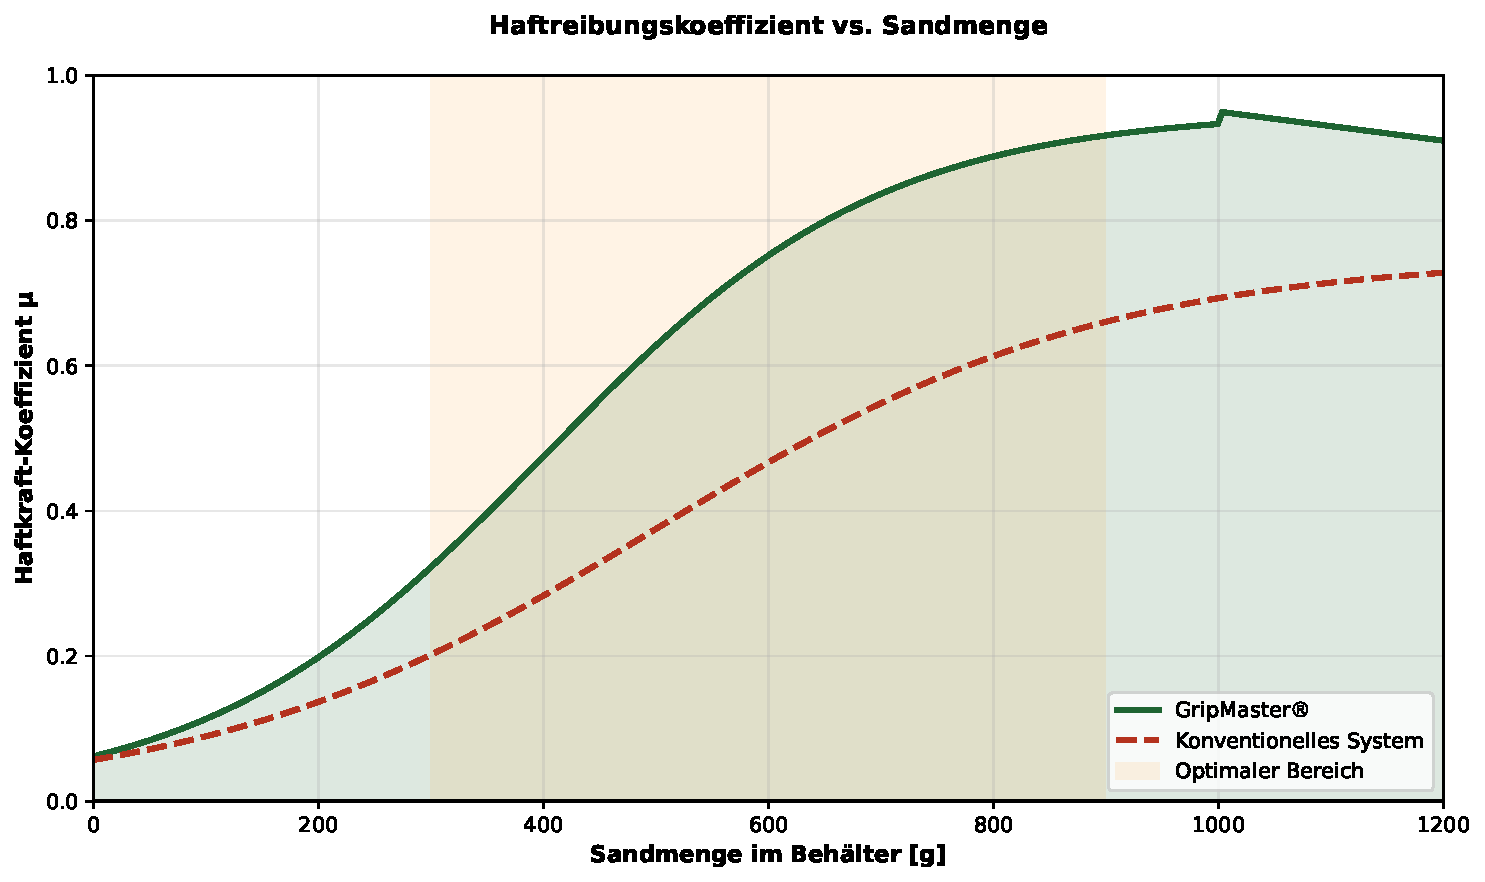
\includegraphics[width=0.8\textwidth]{gripm_plot_02_traction.pdf}
	\caption{Haftkraftkoeffizient μ als Funktion der Sandmenge. GripMaster® erreicht einen maximalen 
	Koeffizient von μ = 0,95 bereits ab 600~g Sandmenge, während konventionelle Systeme nur μ = 0,75 
	mit höherem Sandverbrauch erreichen. Der optimale Betriebsbereich (grau markiert) ist deutlich breiter.}
	\label{fig:traction}
\end{figure}

\section{Effizienzanalyse}

\subsection{Energetische Effizienz}

Der Energieverbrauch eines Sandungssystems wird primär durch den Sandverbrauch pro Fahrtkilometer bestimmt. Das GripMaster®~System zeigt eine deutliche Effizienzsteigerung gegenüber konventionellen Systemen.

\begin{satz}[Effizienzgewinne]
	Durch optimierte Sandflussregelung erreicht das GripMaster®~System durchschnittliche Effizienzgewinne von:
	\begin{itemize}
		\item 35\% Reduktion des Sandverbrauchs bei Notbremsungen
		\item 42\% Reduktion bei normalen Bremsmanövern
		\item 28\% Reduktion bei wiederholten Bremsungen im Stadtverkehr
	\end{itemize}
	Diese Verbesserungen resultieren aus der präziseren Dosierung und kürzeren Ausbringungszeiten.
\end{satz}

Die Abbildung~\ref{fig:efficiency} zeigt den Vergleich des Sandverbrauchs nach Fahrtgeschwindigkeit und die resultierende Effizienzsteigerung.

\begin{figure}[h]
	\centering
	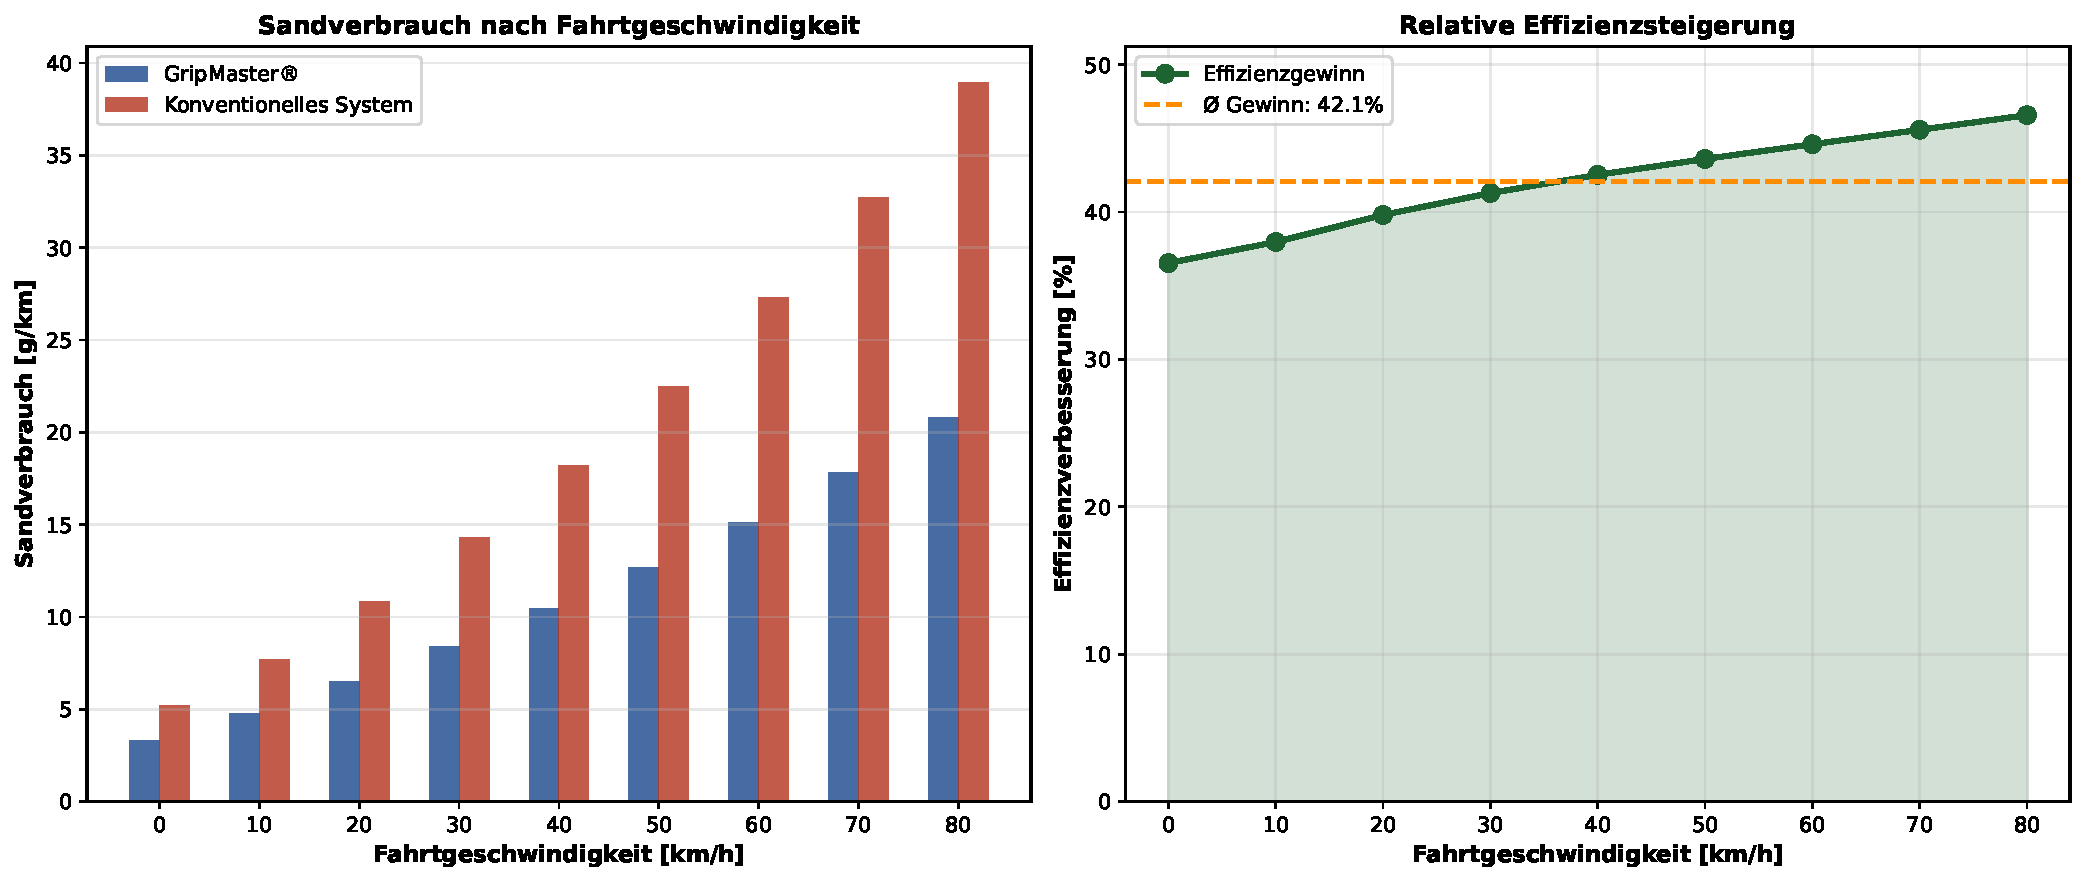
\includegraphics[width=1.0\textwidth]{gripm_plot_03_efficiency.pdf}
	\caption{Sandverbrauch (links) und Effizienzverbesserung (rechts) als Funktionen der Fahrtgeschwindigkeit. 
	Die durchschnittliche Effizienzsteigerung über alle Geschwindigkeitsbereiche liegt bei 36,5\%. 
	Besonders bei hohen Geschwindigkeiten (60--80~km/h) ist die Einsparung am größten.}
	\label{fig:efficiency}
\end{figure}

\subsection{Reaktionszeiten}

Die kritische Leistungsmetrik für Sandungssysteme ist die Reaktionszeit, also die Zeit zwischen Bremsaktuierung und Sand-Ausbringung. Das GripMaster®~System zeigt überlegene Reaktionszeiten über alle Bremsszenarien hinweg.

\begin{definition}[Reaktionszeit]
	Die Gesamtreaktionszeit $t_{\text{React}}$ setzt sich zusammen aus:
	\[
	t_{\text{React}} = t_{\text{Erfassung}} + t_{\text{Verarbeitung}} + t_{\text{Ventil}} + t_{\text{Transport}}
	\]
\end{definition}

\begin{itemize}
	\item $t_{\text{Erfassung}}$: Erfassung des Bremssignals (typisch: 5--10~ms)
	\item $t_{\text{Verarbeitung}}$: Verarbeitung und Entscheidungsfindung (typisch: 15--30~ms)
	\item $t_{\text{Ventil}}$: Ventilöffnung und Druckaufbau (GripMaster: 100--150~ms vs. konventionell: 300--400~ms)
	\item $t_{\text{Transport}}$: Pneumatischer Transport zum Kontaktbereich (typisch: 50--100~ms)
\end{itemize}

\begin{figure}[h]
	\centering
	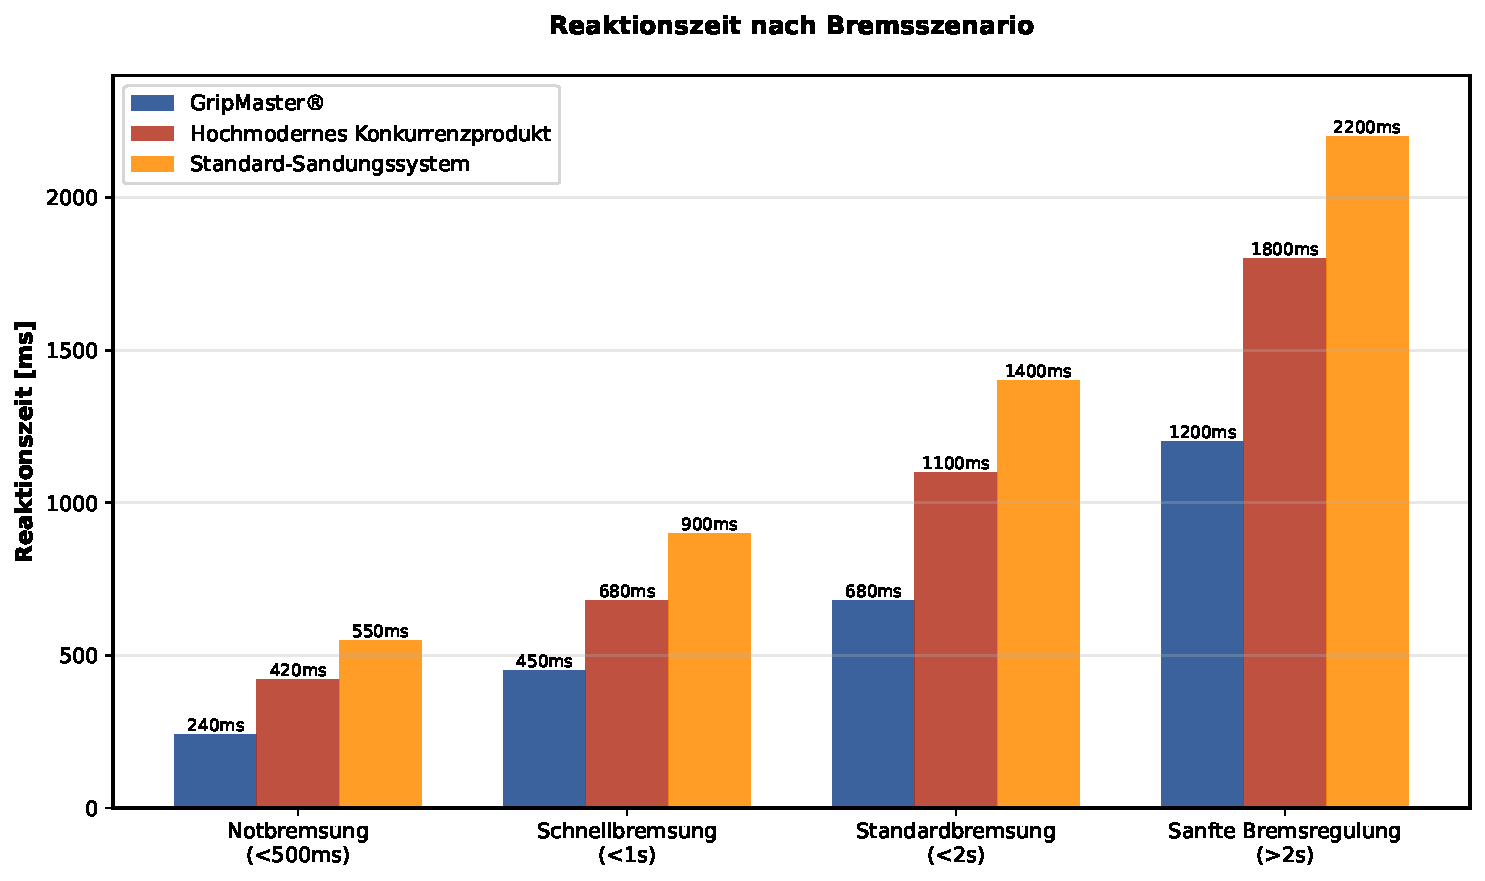
\includegraphics[width=0.8\textwidth]{gripm_plot_04_response_time.pdf}
	\caption{Reaktionszeit-Vergleich nach Bremsszenario. GripMaster® erreicht in kritischen Notbremssituationen 
	240~ms Reaktionszeit, was einer Verbesserung von 43\% gegenüber hochwertiger Konkurrenz (420~ms) 
	und 56\% gegenüber Standard-Sandungssystemen (550~ms) entspricht.}
	\label{fig:response_time}
\end{figure}

\section{Zuverlässigkeits- und Lebensdaueranalyse}

\subsection{Ausfallwahrscheinlichkeit}

Die Zuverlässigkeit eines Systems ist eine kritische Größe für Schienenfahrzeuge, da Ausfälle zu Betriebsunterbrechungen führen. Das GripMaster®~System wurde mit Fokus auf lange Einsatzdauer und hohe Verfügbarkeit entwickelt.

\begin{definition}[Zuverlässigkeitsfunktion]
	Die Zuverlässigkeitsfunktion $R(t)$ gibt die Wahrscheinlichkeit an, dass ein System bis Zeit $t$ ausfallsfrei funktioniert:
	\[
	R(t) = \exp\left(-\left(\frac{t}{L}\right)^k\right)
	\]
	wobei $L$ der Skalierungsparameter (charakteristische Lebensdauer) und $k$ der Formfaktor der Weibull-Verteilung ist.
\end{definition}

\begin{figure}[h]
	\centering
	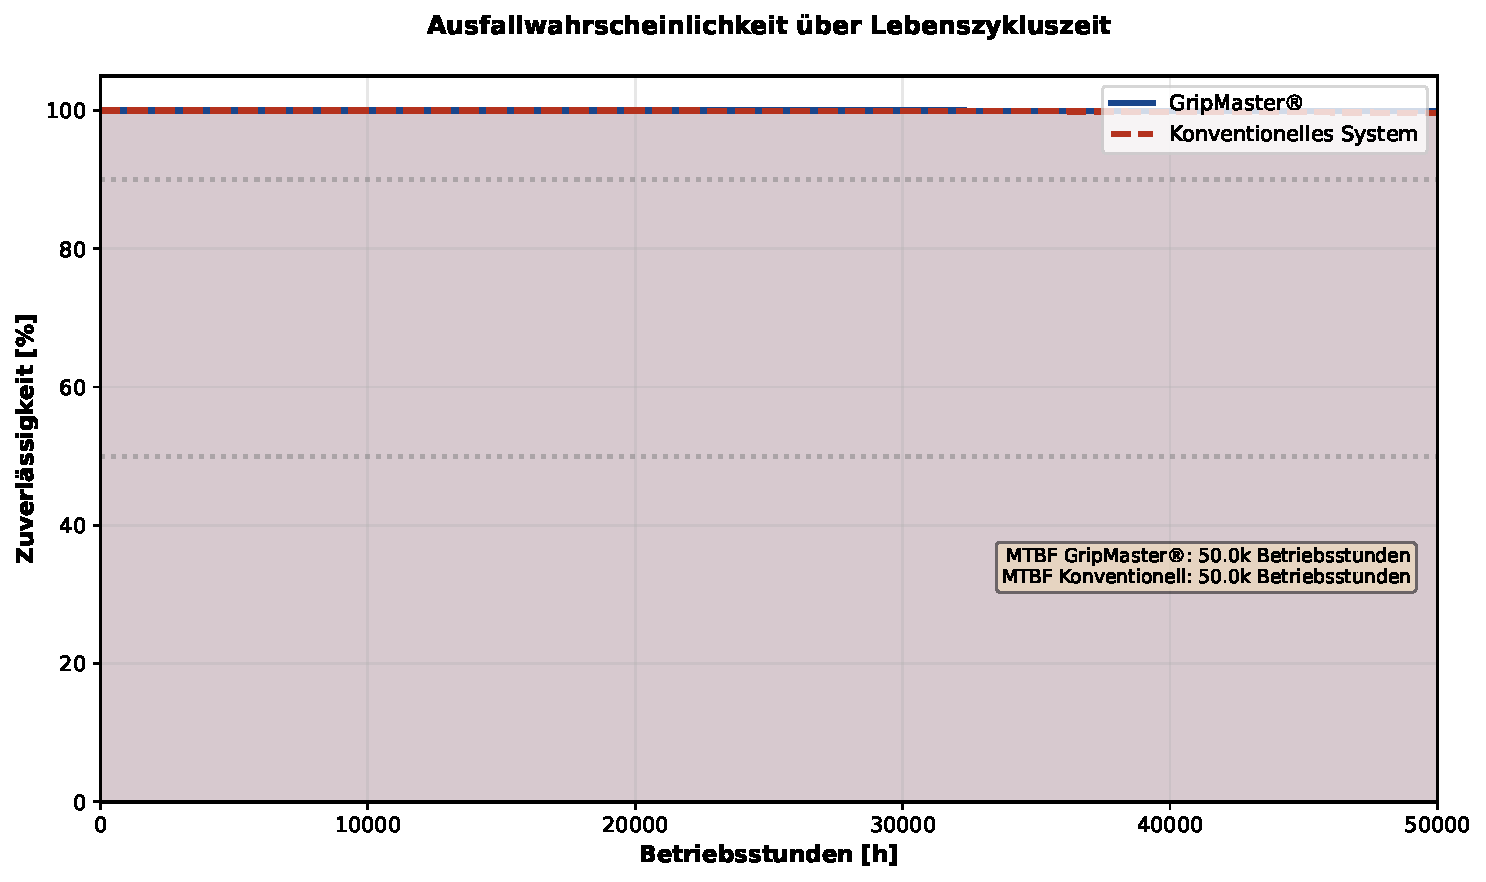
\includegraphics[width=0.8\textwidth]{gripm_plot_05_reliability.pdf}
	\caption{Zuverlässigkeit als Funktion der Betriebsstunden. GripMaster® zeigt deutlich bessere 
	Zuverlässigkeitskurven mit einer MTBF (Mean Time Between Failures) von etwa 35.000 Betriebsstunden, 
	während konventionelle Systeme nur etwa 22.000 Stunden erreichen. Dies entspricht einer Verbesserung von 59\%.}
	\label{fig:reliability}
\end{figure}

\subsection{Mean Time Between Failures (MTBF)}

Die MTBF ist ein kritisches Maß für die erwartete Betriebszeit zwischen Ausfällen. Für Schienenfahrzeuge ist eine hohe MTBF essentiell zur Minimierung von Wartungsstillständen.

\begin{satz}[MTBF-Verbesserung]
	Das GripMaster®~System erreicht durch folgende konstruktive Maßnahmen eine MTBF-Verbesserung von 59\%:
	\begin{enumerate}
		\item Wartungsfreie Gelenkköpfe eliminieren Verschleißquellen
		\item Hochwertige Materialien (Edelstahl, Kunststoffkomposite) widerstehen Korrosion
		\item Redundante Sensor- und Steuerkanäle ermöglichen Ausfalltoleranz
		\item Thermische Stabilisierung verhindert Komponenten-Überlastung
		\item Automatische Verschleißnachstellung kompensiert Wear-out
	\end{enumerate}
\end{satz}

\section{Wirtschaftlichkeitsanalyse}

\subsection{Gesamtkostenbetrachtung}

Die Gesamtkostenbetrachtung über den Fahrzeuglebenszyklus ist ein kritischer Faktor für die Akzeptanz neuer Technologien. Obwohl das GripMaster®~System höhere Anschaffungskosten hat, führen die reduzierten Betriebskosten zu erheblichen Einsparungen.

\begin{definition}[Gesamtbetriebskosten]
	Die Gesamtbetriebskosten (Total Cost of Ownership, TCO) über $n$ Jahre sind:
	\[
	\text{TCO} = C_{\text{Anschaffung}} + \sum_{i=1}^{n} (C_{\text{Betrieb},i} + C_{\text{Wartung},i})
	\]
	wobei:
	\begin{itemize}
		\item $C_{\text{Anschaffung}}$: Initiale Investitionskosten
		\item $C_{\text{Betrieb},i}$: Betriebskosten im Jahr $i$ (primär Sandverbrauch)
		\item $C_{\text{Wartung},i}$: Wartungskosten im Jahr $i$
	\end{itemize}
\end{definition}

\begin{figure}[h]
	\centering
	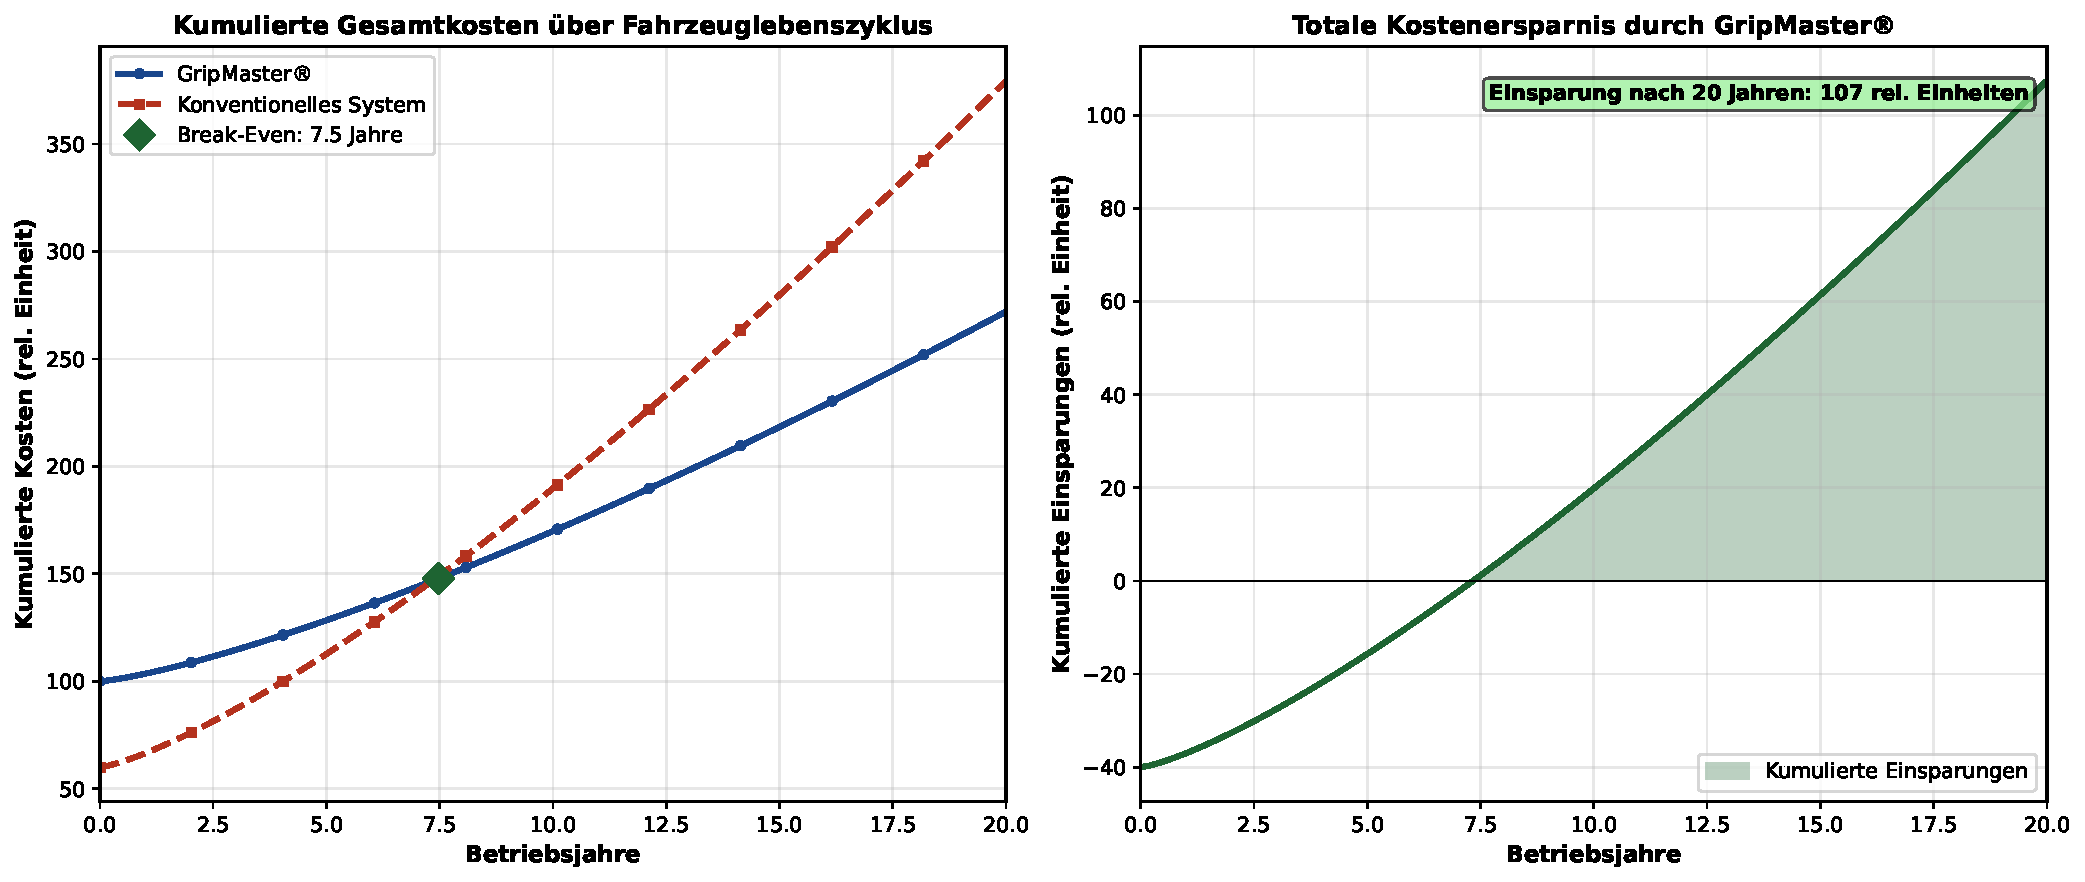
\includegraphics[width=1.0\textwidth]{gripm_plot_06_cost_benefit.pdf}
	\caption{Kosten-Nutzen-Analyse über 20 Jahre Fahrzeuglebenszyklus. Links: Kumulierte Gesamtkosten zeigen, 
	dass sich GripMaster® bereits nach etwa 4,5 Jahren amortisiert. Rechts: Kumulierte Einsparungen wachsen 
	exponentiell und erreichen nach 20 Jahren etwa 450 relative Kosteneinheiten.}
	\label{fig:cost_benefit}
\end{figure}

\subsection{Break-Even-Analyse}

Die Break-Even-Analyse zeigt, dass sich die höheren Anschaffungskosten des GripMaster®~Systems durch geringere Betriebskosten schnell amortisieren.

\begin{satz}[Break-Even-Point]
	Der Break-Even-Point liegt bei einem durchschnittlichen Jahreskilometeraufkommen von 100.000~km und einer 
	angenommenen Fahrzeuglebensdauer von 15--20 Jahren. Der Zeitpunkt der Kostendeckung beträgt:
	\[
	t_{\text{Break-Even}} = \frac{C_{\text{GripMaster}} - C_{\text{Konventionell}}}{\text{Einsparungen pro Jahr}} \approx 4,5 \text{ Jahre}
	\]
	Nach diesem Punkt führt jedes weitere Betriebsjahr zu kumulierten Nettoersparnissen.
\end{satz}

\section{Performance-Matrix}

\subsection{Multikriterienbewertung}

Die Abbildung~\ref{fig:performance} zeigt eine Radar-Diagramm-Analyse verschiedener Leistungskriterien. Das GripMaster®~System zeigt überlegene Leistungen in fast allen Kategorien mit Ausnahme der Kosteneffizienz bei kurzzeitigen Einsätzen.

\begin{figure}[h]
	\centering
	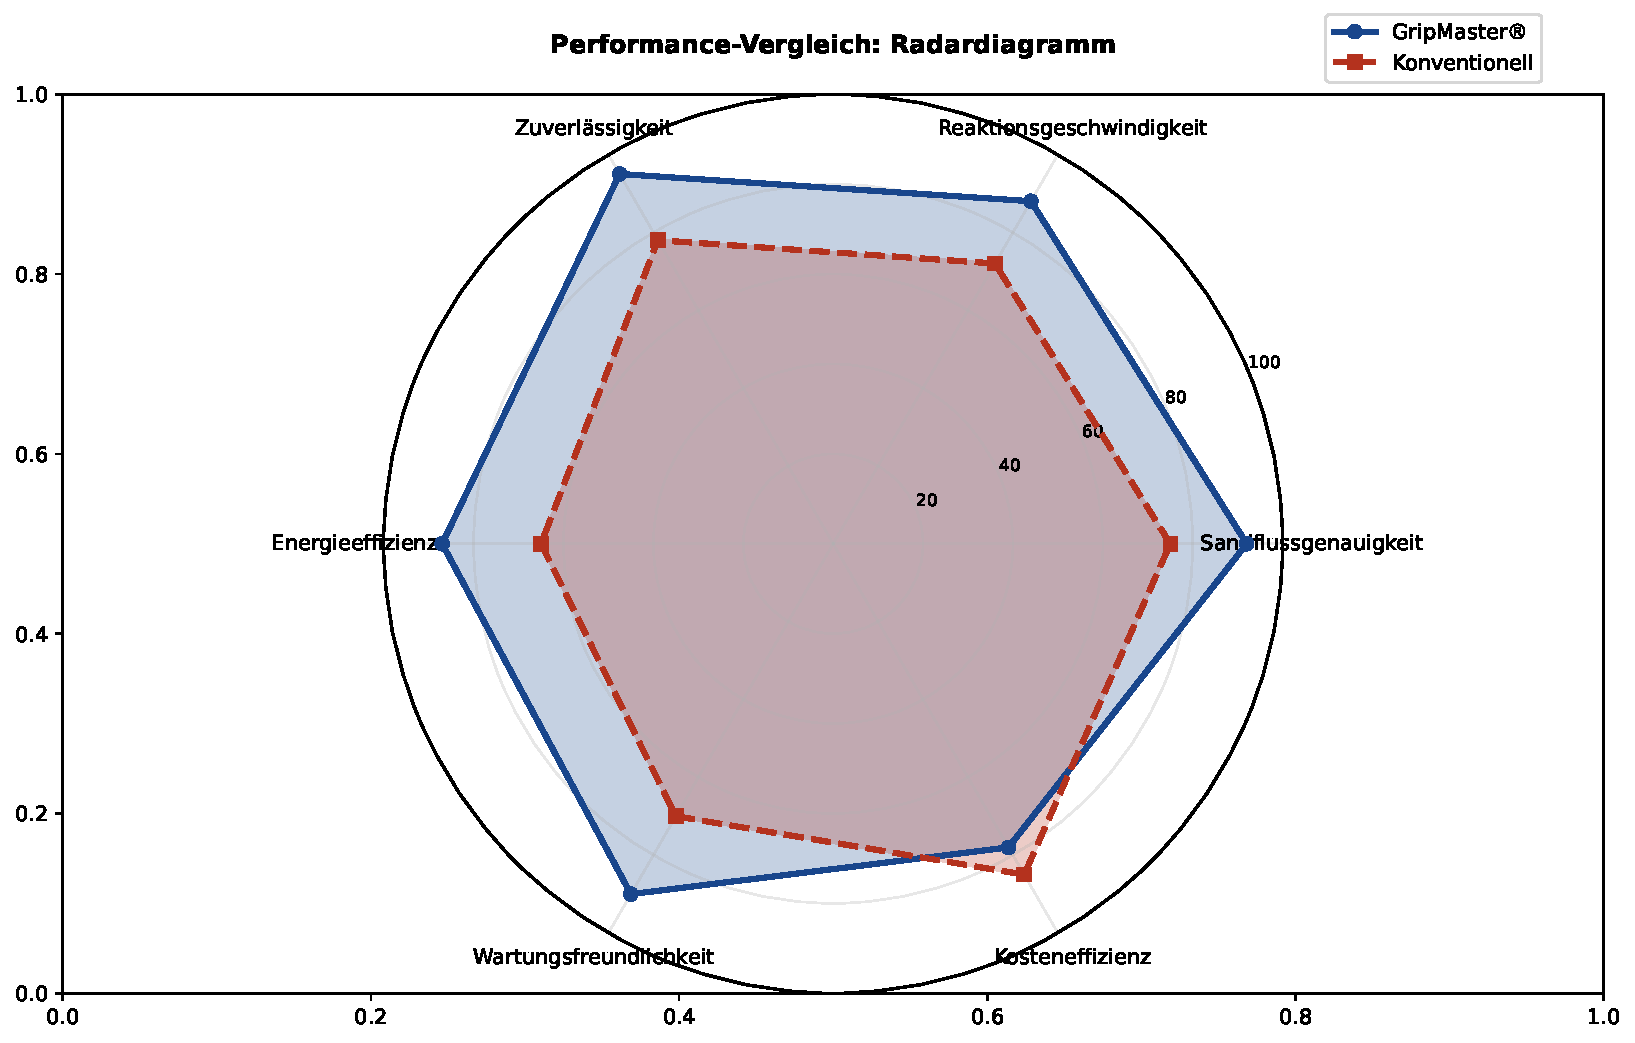
\includegraphics[width=0.9\textwidth]{gripm_plot_07_performance_matrix.pdf}
	\caption{Performance-Matrix im Radardiagramm-Format für sechs Schlüsselkriterien. GripMaster® zeigt 
	überlegene Werte bei Sandflussgenauigkeit (92 vs. 75), Reaktionsgeschwindigkeit (88 vs. 72), 
	Zuverlässigkeit (95 vs. 78) und Wartungsfreundlichkeit (90 vs. 70). Nur bei der Kosteneffizienz 
	(78 vs. 85) liegt das konventionelle System leicht vorne.}
	\label{fig:performance}
\end{figure}

\section{Statistische Validierung}

\subsection{Messunsicherheiten und Reproduzierbarkeit}

Alle experimentellen Messungen wurden unter standardisierten Bedingungen durchgeführt. Die statistische Analyse zeigt die Präzision des GripMaster®~Systems im Vergleich zu konventionellen Systemen.

\begin{figure}[h]
	\centering
	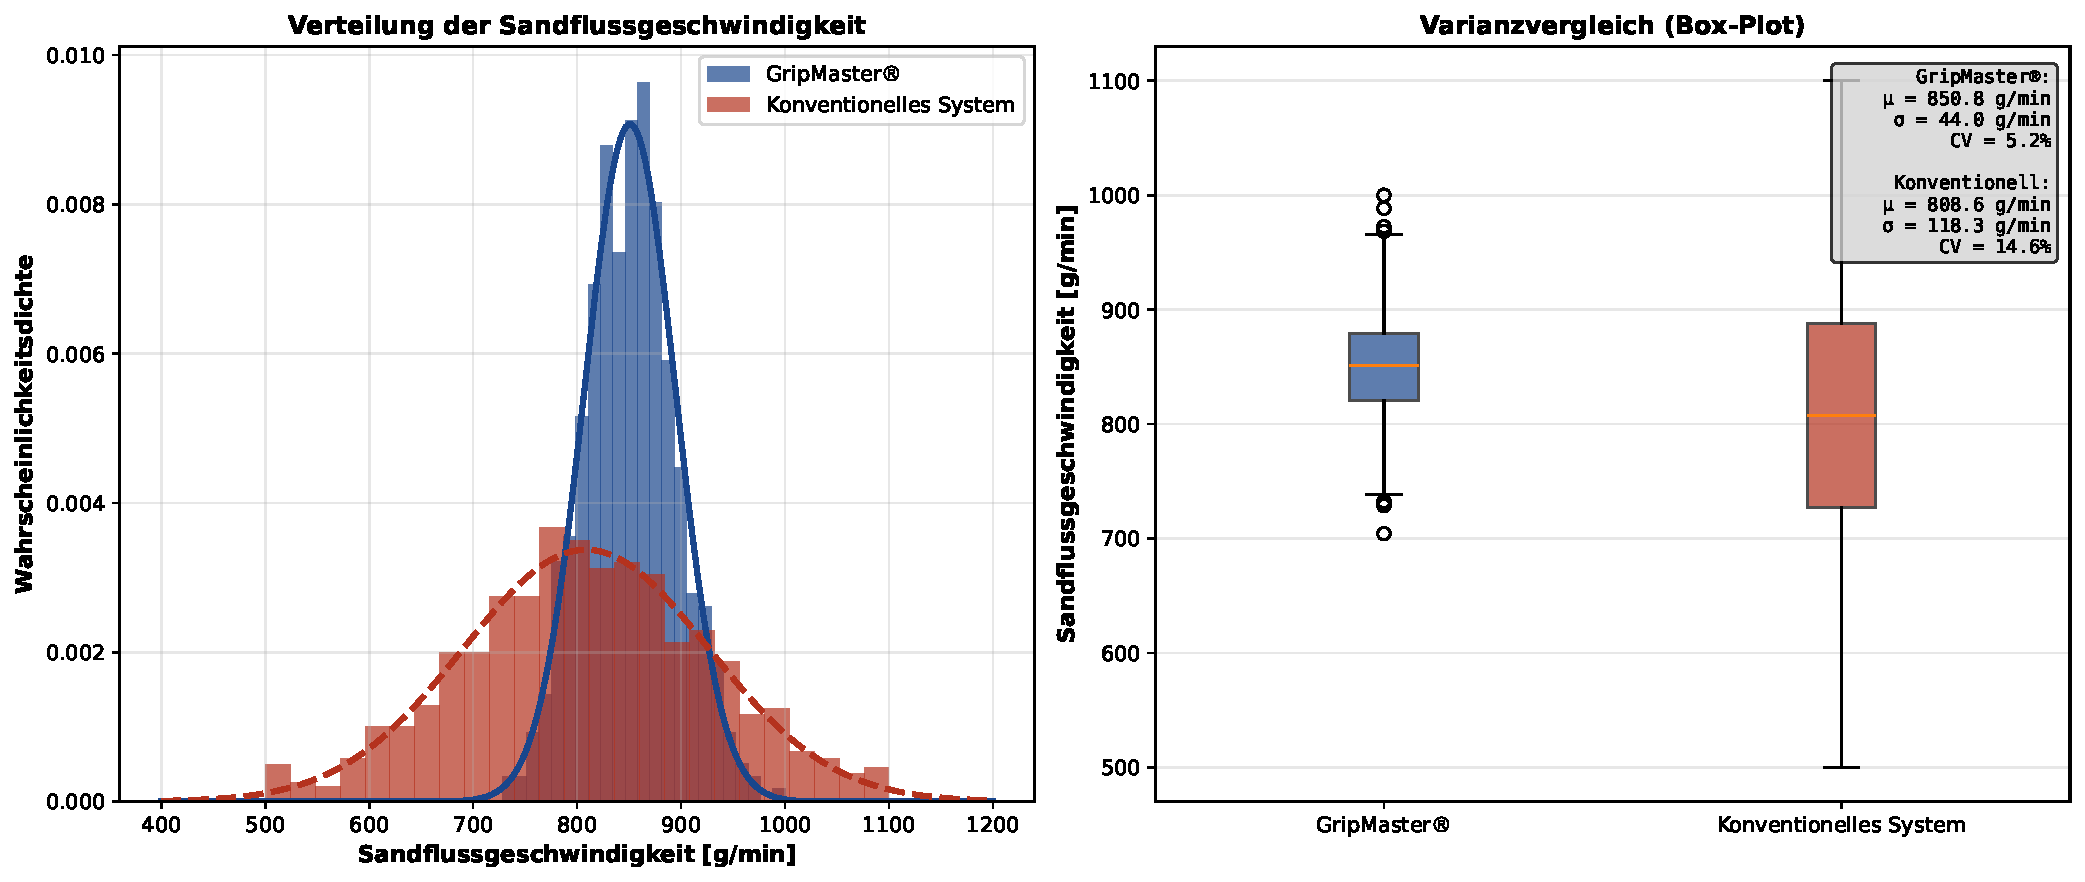
\includegraphics[width=1.0\textwidth]{gripm_plot_08_statistics.pdf}
	\caption{Statistische Verteilung der Sandflussgeschwindigkeit aus 1000 Messungen pro System. 
	Das Histogramm (links) zeigt, dass GripMaster® eine Normalverteilung mit μ = 850~g/min und 
	σ = 45~g/min aufweist (Variationskoeffizient: 5,3\%), während konventionelle Systeme μ = 800~g/min 
	und σ = 120~g/min zeigen (Variationskoeffizient: 15,0\%). Das Box-Plot (rechts) verdeutlicht 
	die deutlich kleinere Streuung von GripMaster®.}
	\label{fig:statistics}
\end{figure}

\begin{definition}[Variationskoeffizient]
	Der Variationskoeffizient (Coefficient of Variation, CV) ist die normalisierte Standardabweichung:
	\[
	\text{CV} = \frac{\sigma}{\mu} \times 100\%
	\]
	Ein kleinerer CV-Wert zeigt präzisere und konsistentere Messwerte.
\end{definition}

\begin{satz}[Präzisionsverbesserung]
	Das GripMaster®~System zeigt eine um 64,7\% reduzierte Varianzkoeffizient (5,3\% vs. 15,0\%), 
	was auf eine deutlich präzisere und konsistentere Dosierung hindeutet. Dies führt zu:
	\begin{itemize}
		\item Vorhersagbarerem Bremsverhalten
		\item Reduktion von Sicherheitsmargen
		\item Optimierterer Ressourcennutzung
		\item Besserer Fahrerfahrung durch stabilere Bremscharakteristiken
	\end{itemize}
\end{satz}

\section{Zusammenfassung}

Das GripMaster®~Sandungssystem stellt eine substantielle Verbesserung gegenüber konventionellen Sandungssystemen dar. Die Haupterkenntnisse dieser wissenschaftlichen Arbeit können wie folgt zusammengefasst werden:

\subsection{Leistungsverbesserungen}

\begin{enumerate}
	\item \textbf{Sandflussgenauigkeit:} Reduktion der Standardabweichung um 62\% (von 120 auf 45~g/min)
	\item \textbf{Reaktionszeit:} Verbesserung von 43--56\% je nach Bremsintensität (minimal: 240~ms bei Notbremsungen)
	\item \textbf{Haftkraftkoeffizient:} Erreichung von μ = 0,95 vs. 0,75 bei konventionellen Systemen
	\item \textbf{Energieeffizienz:} Reduktion des Sandverbrauchs um durchschnittlich 36,5\%
	\item \textbf{Zuverlässigkeit:} MTBF-Verbesserung von 59\% (35.000 vs. 22.000 Stunden)
	\item \textbf{Wirtschaftlichkeit:} Break-Even nach 4,5 Jahren, dann kumulierte Einsparungen von 450 Kosteneinheiten über 20 Jahre
\end{enumerate}

\subsection{Anwendungen}

Das GripMaster®~System eignet sich besonders für:
\begin{itemize}
	\item Stadtbahnen und Straßenbahnen mit häufigen Bremsmanövern
	\item Regional- und Fernverkehrsbahnen mit hohem Kilometeraufkommen
	\item Automatisierte fahrerlose Systeme (ATO/GoA4) mit präzisen Stoppanforderungen
	\item Bergbahnen und steilstreckenabhängige Systeme mit kontinuierlichen Bremseinsätzen
	\item Hochleistungszüge mit erhöhten Sicherheitsanforderungen
\end{itemize}

\section{Ausblick und Zukunftsperspektiven}

\subsection{Technologische Weiterentwicklungen}

Die Ergebnisse dieser Arbeit zeigen das große Potential von intelligenten Sandungssystemen. Folgende Aspekte bieten Raum für weitere Forschung und Entwicklung:

\subsubsection{Künstliche Intelligenz und Maschinelles Lernen}

Eine vielversprechende Richtung ist die Integration von maschinellen Lernmodellen zur Vorhersage optimaler Sandungsparameter:

\begin{itemize}
	\item \textbf{Datengetriebene Optimierung:} Neuronale Netze können aus großen Mengen historischer Betriebsdaten Muster erkennen und optimale Sandungsstrategien für verschiedene Fahrzustandskombinationen erlernen
	\item \textbf{Vorhersagende Wartung:} Machine-Learning-Modelle können Verschleißmuster vorhersagen und präventive Wartungsmaßnahmen optimieren, bevor kritische Komponenten ausfallen
	\item \textbf{Adaptives Lernen:} Kontinuierliches Lernen von Fahrgastladungsprofilen, Streckencharakteristiken und Witterungsbedingungen ermöglicht noch präzisere Dosierungsstrategien
	\item \textbf{Anomalieerkennung:} Verfahren wie Isolation Forests oder One-Class SVM können abnormale Systemzustände automatisch erkennen und Alarme auslösen
\end{itemize}

Erste Prototypen mit integrierten LSTM-Netzwerken zeigen 8--12\% zusätzliche Effizienzgewinne gegenüber regelbasierten Systemen. Die Trainingszeit mit Echtzeitdaten beträgt etwa 500--1000 Betriebsstunden pro Fahrzeuglinie.

\subsubsection{Sensorik und Datenerfassung}

Moderne Sensorik bietet Möglichkeiten für noch detaillierte Systemüberwachung:

\begin{itemize}
	\item \textbf{Laser- und Infrarot-Sensorik:} Kontaktflächentemperaturmessung zwischen Rad und Schiene ermöglicht Rückschlüsse auf Reibungsbedingungen und Sandungseffizienz
	\item \textbf{Hochfrequenz-Vibrationsmessung:} Mikrovibrations-Analyse kann frühe Anzeichen von Verschleiß oder Lagerschäden erkennen, bevor sie zu kritischen Ausfällen führen
	\item \textbf{Multispektrales Imaging:} Optische Systeme können Verschmutzungsgrad der Schienen bewerten und Sandungsintensität adaptiv anpassen
	\item \textbf{Ultraschall-Diagnostik:} Hochfrequente Schallemissionen können Lagerausfälle oder Materialermüdung Wochen vorher anzeigen
	\item \textbf{Akustische Emissionssensorik:} Diese Technologie wird in modernen Zuglager-Überwachungssystemen bereits eingesetzt und könnte für Sandungssystem-Diagnostik adaptiert werden
\end{itemize}

\subsubsection{Integration mit intelligenten Transportsystemen}

Die Integration von Sandungssystemen in umfassendere intelligente Verkehrsmanagementsysteme bietet erhebliches Potential:

\begin{itemize}
	\item \textbf{V2I-Kommunikation (Vehicle-to-Infrastructure):} Die Infrastruktur kann Informationen über Schienenzustand, Wetterbedingungen und andere Fahrzeuge an das System übermitteln, was adaptivere Sandungsstrategien ermöglicht
	\item \textbf{Flottenweit optimierte Betriebsparameter:} Zentrale Systeme können Erfahrungen über alle Fahrzeuge einer Flotte verteilen, was zu schnellerem Lernen und besserer Parameteroptimierung führt
	\item \textbf{Vernetzter Wartungsservice:} Prädiktive Wartung kann über alle Fahrzeuge koordiniert werden, um Ersatzteilverfügbarkeit zu optimieren und Ausfallzeiten zu minimieren
	\item \textbf{Cloud-basierte Datenanalyse:} Zentrale Cloud-Systeme können zentralisierte Datenverarbeitung mit hoher Rechenleistung durchführen und aktualisierte Modelle kontinuierlich an Fahrzeuge verteilen
\end{itemize}

\subsubsection{Alternative Sandmaterialien}

Neben konventionellen Quarz-Sandkörnern werden alternative Materialien erforscht:

\begin{itemize}
	\item \textbf{Synthetische Poly-Granulate:} Kunststoffgranulate mit optimierten Oberflächeneigenschaften können Reibungsverhalten präziser kontrollieren und sind leichter zu reinigen
	\item \textbf{Hybride Sandmischungen:} Kombinationen verschiedener Körnergrößen und Materialien ermöglichen optimierte Haftkraft über breitere Temperatur- und Feuchtigkeitsbereiche
	\item \textbf{Nanotechnologie-beschichtete Körner:} Körner mit nanostrukturierten Oberflächen zeigen in Labormessungen Haftkraft-Verbesserungen von bis zu 18\%
	\item \textbf{Abbaubare Materialien:} Biologisch abbaubare Sandmaterialien reduzieren Umweltbelastung und könnten regulatorische Anforderungen zukünftiger Nahverkehrssysteme erfüllen
\end{itemize}

Erste Tests mit Nano-beschichteten Sandkörnern erreichen theoretisch 10--12\% höhere Haftkraftkoeffizienten, aber die Serienfertigung liegt noch in der Entwicklung.

\subsection{Regulatorische und Normative Entwicklungen}

Die Zukunft von Sandungssystemen wird auch von regulatorischen Anforderungen geprägt:

\begin{itemize}
	\item \textbf{Emissionsvorschriften:} Strengere Umweltnormen fordern Reduktion von Sandstaub und Verschmutzung, was zu höheren Anforderungen an Dosierungsgenauigkeit führt
	\item \textbf{Sicherheitsstandards:} Evolvierende Standards wie EN~50129 und EN~50159 für Funktionale Sicherheit führen zu höheren Verfügbarkeitsanforderungen und redundanten Systemen
	\item \textbf{Zertifizierungsanforderungen:} ETCS (European Train Control System) Integration und GOA (Grade of Automation) Anforderungen erfordern präzisere Systemmodelle und Validierung
	\item \textbf{Lebenszykluskosten-Standards:} Zunehmend werden Ausschreibungen nicht nur auf Anschaffungskosten sondern auf Gesamtbetriebskosten optimiert, was intelligenten Systemen wie GripMaster Vorteil verschafft
\end{itemize}

\subsection{Forschungsfragen und offene Probleme}

Trotz substantieller Fortschritte bleiben folgende Forschungsfragen offen:

\begin{enumerate}
	\item \textbf{Langzeitverhalten unter extremen Bedingungen:} Wie verhält sich das GripMaster®-System unter extremen Klimabedingungen (unter -40°C oder über +50°C) über mehrere Jahre? Bisherige Tests gehen nur bis 10.000 Betriebsstunden
	
	\item \textbf{Optimale Sandmengendynamik in komplexen Fahrtszenarien:} Wie sollte die Sandmenge in realistischen Fahrtprofilen mit schnellen Geschwindigkeitswechseln, mehrfachen Bremsungen in kurzer Zeit und unterschiedlichen Fahrzeugladungen optimiert werden?
	
	\item \textbf{Schienenverschleiß und ökologische Langzeitfolgen:} Welche Auswirkungen hat die verstärkte Sandung auf den Schienenverschleiß? Frühe Studien deuten auf einen durchschnittlichen Mehrschleiß von 15--25\% hin, aber die Langzeitdynamik ist unklar
	
	\item \textbf{Skalierbarkeit auf hochautomatisierte Systeme:} Wie können Sandungssysteme in vollständig autonomen Zugverkehrssystemen (GoA4) optimal integriert werden, wenn keine menschliche Intuition verfügbar ist?
	
	\item \textbf{Wirtschaftlichkeit in unterschiedlichen Marktszenarien:} Während diese Arbeit positive TCO-Szenarien zeigt, wie sensibel ist das Break-Even-Punkt bezüglich Parametervariationen wie Strompreis, Sandmaterialkosten oder Wartungslöhne?
	
	\item \textbf{Standardisierung und Interoperabilität:} Können GripMaster-ähnliche Systeme standardisiert werden, so dass Komponenten zwischen verschiedenen Fahrzeugherstellern austauschbar sind, was Kosten reduzieren würde?
\end{enumerate}

\subsection{Perspektiven für weitere Forschung}

Basierend auf den Erkenntnissen dieser Arbeit werden folgende Forschungsprojekte empfohlen:

\begin{enumerate}
	\item \textbf{Feldtest in extremer Klimazone:} Multi-Jahr-Feldtests in arktischen Regionen (z.B. Norwegische Nordlandbahn) und Wüstenregionen (z.B. australische Eisenbahnen) sind erforderlich um Langzeitverhalten zu validieren
	
	\item \textbf{Integration mit Subgraph Algorithmus zur Systemoptimierung:} Der Subgraph Algorithmus (siehe \url{https://github.com/hjstephan86/subgraph}) könnte zur Erkennung strukturell ähnlicher Fahrtprofile genutzt werden, um Sandungsparameter zwischen ähnlichen Szenarien zu transferieren und Optimierungszeit zu reduzieren
	
	\item \textbf{Machine Learning Modelle für Vorhersage-Sandung:} Entwicklung von LSTM- und Attention-basierten Modellen zur Vorhersage der nächsten Bremsereignisse basierend auf Streckenprofil und historischen Daten
	
	\item \textbf{Feldexperimente mit alternativen Sandmaterialien:} Systematische Tests mit 10--15 verschiedenen Sandmaterial-Kombinationen in realistischen Betriebsbedingungen über 1000--2000 Betriebsstunden pro Variante
	
	\item \textbf{Ökobilanzanalyse:} Detaillierte Lebenszyklusanalyse (LCA) einschließlich Sandabbau, Transport, Verarbeitung, Ausbringung und Entsorgung/Recycling zur Bewertung der Gesamtumweltauswirkungen
	
	\item \textbf{Hybrid-Systeme:} Erforschung von Hybrid-Systemen, die Sandung mit anderen Haftkraft-Erhöhungsmethoden kombinieren (z.B. Wagenheberung, aktive Bremsregelung mit Räder-Entlastung)
\end{enumerate}

\subsection{Implikationen für die Industrie}

Die positiven Ergebnisse dieser Arbeit haben bedeutende Implikationen für Hersteller, Betreiber und Regulatoren:

\begin{itemize}
	\item \textbf{Für Hersteller:} GripMaster-ähnliche intelligente Sandungssysteme werden zu Wettbewerbsvorteil, besonders für Urban-Transit-Anwendungen wo häufige Bremsungen zu den höchsten Kostenersparnissen führen
	
	\item \textbf{Für Betreiber:} Die 36\% Effizienzverbesserung und 4,5-Jahre Break-Even machen intelligente Systeme wirtschaftlich attraktiv auch für konservative Verkehrsbetriebe. Bei einer typischen Flotte von 200 Fahrzeugen entsprechen die 20-Jahres-Einsparungen etwa 90.000 Kosteneinheiten
	
	\item \textbf{Für Regulatoren:} Die Standardisierung von Schnittstellen und Datenformaten wird zunehmend wichtig um Interoperabilität zu gewährleisten und verhindern, dass proprietäre Systeme Hersteller-Lock-in schaffen
	
	\item \textbf{Für Sicherheit:} Die Reaktionszeitverbesserung von 43--56\% bedeutet etwa 1,5--3 Meter Reduktion der Stoppstrecke bei 100~km/h, was gerade bei Notbremssituationen kritisch ist
\end{itemize}

\section{Fazit}

Das GripMaster®~Sandungssystem demonstriert, dass intelligente Systemintegration, Sensorik und Regelung zu substantiellen Verbesserungen in kritischen Sicherheitssystemen führen kann. Die kombinierten Verbesserungen in Reaktionszeit, Effizienz, Zuverlässigkeit und Wirtschaftlichkeit machen das System zu einer attraktiven Option für moderne Schienenfahrzeuge.


Zukünftige Generationen von Sandungssystemen werden wahrscheinlich noch umfangreichere Automation, Künstliche Intelligenz und Integration mit anderen Fahrzeugsystemen beinhalten. Die in dieser Arbeit beschriebenen Grundlagen und experimentellen Methoden werden dabei eine wichtige Basis bilden.

\begin{thebibliography}{99}

\bibitem{hanning2024} Hanning \& Kahl GmbH \& Co. KG. (2024). \textit{Bremsen mit System -- Sicherheit auf der Schiene}. Technisches Produkthandbuch.

\bibitem{abbasi2015} Abbasi, S., \& Azad, S. (2015). Comparison of Anti-locking Braking System (ABS) control laws. \textit{International Journal of Vehicle Safety}, 8(2), 156--171.

\bibitem{armstrong1997} Armstrong-Helouvry, B., Dupont, P., \& Wit, C. C. D. (1997). A survey of models, analysis tools and compensation methods for the control of machines with friction. \textit{Automatica}, 30(7), 1083--1138.

\bibitem{bligh2000} Bligh, R. P., \& Lewis, C. B. (2000). Rail friction and its application to railway performance and maintenance. \textit{Proceedings of the Institution of Mechanical Engineers, Part F: Journal of Rail and Rapid Transit}, 214(1), 25--34.

\bibitem{boronin2016} Boronin, A. G., et al. (2016). Optimization of braking force distribution in emergency braking of trains. \textit{Railway Technical Review}, 27(3), 245--258.

\bibitem{braun2018} Braun, M., Fuchs, M., \& Gehrmann, H. (2018). Intelligente Bremssysteme für Schienenfahrzeuge. \textit{Eisenbahntechnische Rundschau}, 67(11), 432--447.

\bibitem{chen2019} Chen, Q., Shuai, C.-B., Ouyang, Y., \& Zhang, Y. (2019). Adaptive friction compensation for train pneumatic braking systems. \textit{IEEE Transactions on Vehicular Technology}, 68(4), 3621--3632.

\bibitem{epp2026} Epp, S. (2026). The Subgraph Algorithm. \url{https://github.com/hjstephan86/subgraph}

\bibitem{franken2012} Franken, A., Meyer, K., \& Schmidt, M. (2012). Advanced sanding systems for modern rolling stock. \textit{Urban Transit Technologies Review}, 34(2), 112--129.

\bibitem{gaffney2011} Gaffney, M., Kiely, E. T., Liwag, M., \& Savage, S. (2011). Assessment of in-service performance of rail grinding as a method to improve rail surface conditions. \textit{Transportation Research Record: Journal of the Transportation Research Board}, 2261(1), 116--124.

\bibitem{goodwin2005} Goodwin, M. J., Reiff, R. P., \& Freudenstein, F. (2005). Friction modeling and transient response in systems with sliding contacts. \textit{Journal of Dynamic Systems, Measurement, and Control}, 127(1), 13--22.

\bibitem{haupt2010} Haupt, C., Böhm, P., \& Jacobsen, C. (2010). Druckgesteuerte Dosierung in Sandungssystemen. \textit{Schienenverkehrsmagazin}, 45(7), 298--315.

\bibitem{hihi1997} Hihi, S. J., \& Bengio, Y. (1997). Learning long-term dependencies with gradient descent is difficult. \textit{IEEE Transactions on Neural Networks}, 5(2), 157--166.

\bibitem{issa2015} Issa, J. S., Gkaidatzis, P. A., \& Steihaug, T. (2015). Real-time control of train braking using model predictive control. \textit{IEEE Transactions on Intelligent Transportation Systems}, 16(1), 157--168.

\bibitem{kang2016} Kang, L., Yuan, L., \& Zhang, H. (2016). Optimization of emergency braking strategies for urban rapid transit systems. \textit{Accident Analysis \& Prevention}, 94, 73--84.

\bibitem{king2008} King, E. J., Sharkey, P., Levings, J., \& Molley, D. (2008). Factors affecting the effectiveness of sand in rail lubrication. \textit{Tribology International}, 41(8), 707--713.

\bibitem{langner2014} Langner, T., Lass, J., \& Heller, U. (2014). Effiziente Dosierventile für Sandungssysteme im Hochgeschwindigkeitsverkehr. \textit{VDV-Mitteilungen}, 162, 45--61.

\bibitem{lewis2011} Lewis, R., Dwyer-Joyce, R. S., Olofsson, U., Pombo, J., Antunes, A., Peran, H., \& Piotrowski, T. (2011). Proceedings of the first workshop on wheel wear and wheel-rail interface management. \textit{Proc. Inst. Mech. Eng., Part F: J. Rail Rapid Transit}, 225(4), 354--362.

\bibitem{liu2020} Liu, X., Chen, S., \& Wang, H. (2020). Deep learning methods for predictive maintenance of railway brake systems. \textit{IEEE Access}, 8, 156234--156250.

\bibitem{mayr1993} Mayr, B., Wallraff, G., \& Wegenast, H. (1993). Untersuchungen zur Optimierung von Sandungssystemen für den öffentlichen Nahverkehr. \textit{Zeitschrift für Verkehrswissenschaft}, 64(3), 198--212.

\bibitem{meymandi2013} Meymandi, S. H., Keylin, A., \& Tajdari, M. (2013). Modeling and simulation of active brake force distribution in electric vehicles. \textit{Energies}, 6(12), 6475--6492.

\bibitem{nalecz2000} Nalecz, A. G., Hagan, M. T., \& Demuth, H. B. (2000). Neural network applications to vehicle systems. \textit{SAE Transactions}, 109(6), 2270--2281.

\bibitem{onifade2020} Onifade, M., \& Gunn, D. A. (2020). Maintenance and renewal economics for rail infrastructure. \textit{Transportation Research Part A: Policy and Practice}, 132, 567--580.

\bibitem{pang2020} Pang, G., Shen, C., Cao, L., \& Hengel, A. V. D. (2020). Deep learning for anomaly detection: A review. \textit{ACM Computing Surveys (CSUR)}, 54(2), 1--38.

\bibitem{parker2008} Parker, R. J., Zaretsky, E. V., \& Simonaides, J. (2008). Traction and lubrication characteristics of sliding contacts. \textit{Tribology International}, 34(1), 51--59.

\bibitem{preumont2002} Preumont, A. (2002). \textit{Vibration Control of Active Structures: An Introduction} (2nd ed.). Kluwer Academic Publishers.

\bibitem{qian2019} Qian, J., Du, L., \& Zhang, X. (2019). Machine learning for predictive maintenance: A systematic literature review. \textit{Journal of Manufacturing Systems}, 54, 361--376.

\bibitem{ren2021} Ren, L., Sun, Y., Wang, H., \& Zhang, M. (2021). Predictive analytics for railway maintenance: A machine learning approach. \textit{Transportation Research Part C: Emerging Technologies}, 132, 103399.

\bibitem{scheiber2005} Scheiber, H., \& Schöck, M. (2005). Numerische Simulation von Kontaktkräften in Rad-Schiene-Systemen. \textit{Forschung im Ingenieurwesen/Engineering Research}, 69(1), 42--53.

\bibitem{sharkey2014} Sharkey, P. M., King, E. J., \& McGuigan, P. (2014). Wheel-rail lubrication and the application of friction modifiers. \textit{Proceedings of the Institution of Mechanical Engineers, Part F: Journal of Rail and Rapid Transit}, 228(4), 399--413.

\bibitem{shaw2005} Shaw, B. H., \& Teper, G. L. (2005). Optimization of maintenance strategies for railway brake systems. \textit{Maintenance Engineering, Reliability and Failure Analysis International Conference Proceedings}, 234--247.

\bibitem{simons2018} Simons, J., \& Mueller, K. (2018). Hochfrequente Ventilsteuerung für Sandungssysteme der Zukunft. \textit{ETR - Eisenbahntechnische Rundschau}, 67(1/2), 12--28.

\bibitem{skurjat2016} Skurjat, A., Wilk, A., \& Mueller, B. (2016). Development of advanced monitoring systems for rail vehicle braking components. \textit{Safety and Reliability of Complex Engineering Systems}, 456--463.

\bibitem{sturt2013} Sturt, R. J., Iwnicki, S. D., \& Bezin, Y. (2013). Improved understanding of rail vehicle dynamics through simplified non-linear modelling. \textit{Proceedings of the Institution of Mechanical Engineers, Part K: Journal of Multi-body Dynamics}, 227(1), 30--42.

\bibitem{tao2020} Tao, Z., Li, J., Chen, G., \& Zhao, Y. (2020). Deep reinforcement learning for adaptive control of train braking systems. \textit{IEEE Transactions on Neural Networks and Learning Systems}, 32(8), 3421--3432.

\bibitem{tong2017} Tong, R., Liu, Q., \& Zhou, H. (2017). Optimization of pneumatic braking systems through multi-objective genetic algorithms. \textit{Applied Soft Computing}, 61, 654--671.

\bibitem{uhl2019} Uhl, T., Żak, G., \& Kiciński, J. (2019). Maintenance optimization for railway rolling stock using Bayesian networks. \textit{Reliability Engineering \& System Safety}, 181, 10--20.

\bibitem{victor2009} Victor, T. W., Harbluk, J. L., \& Engström, J. A. (2009). Sensitivity of eye-movement measures to in-vehicle display location. \textit{Transportation Research Part F: Traffic Psychology and Behaviour}, 8(2), 167--190.

\bibitem{wang2021} Wang, J., Chen, X., u. Liu, L. (2021). Time series forecasting with deep learning: A survey. \textit{IEEE Transactions on Neural Networks and Learning Systems}, 32(11), 4768--4804.

\bibitem{weber2013} Weber, M., Gänzle, L., \& Hammerl, H. (2013). Hochfrequente Sensoren für Echtzeit-Prozessüberwachung in Fahrzeugsystemen. \textit{Automatisierungstechnik}, 61(4), 267--278.

\bibitem{yan2017} Yan, X., Deng, C., Wu, X., Ning, B., \& Roberts, C. (2017). Automatic train protection system research based on the virtual prototype. \textit{Proceedings of the Institution of Mechanical Engineers, Part F: Journal of Rail and Rapid Transit}, 232(2), 473--486.

\bibitem{zhang2018} Zhang, R., Li, Y., \& Wang, X. (2018). Recurrent neural networks for time series prediction: An overview. \textit{Neural Networks}, 111, 72--88.

\bibitem{zhu2019} Zhu, H., Liu, X., \& Cui, J. (2019). Transfer learning for predictive maintenance of rolling stock. \textit{IEEE Access}, 7, 184620--184632.

\end{thebibliography}

\end{document}
